%This is the experiment section of my Master Thesis
\section{Experiments}\label{experiments}
In this section, the work that has been done will be explained. \\
The experiments has been carried out with both male and female voices, and two different methods have been applied (Dependent models, section \ref{dpm}, Adaptation, section \ref{adapt}) in order to get the synthesized voices (section \ref{synt}).\\
Rergarding the vocoder, GlottHMM has been used and then the results have been compared with STRAIGHT vocoder (see \ref{results}).\\
\subsection{Depenent models}\label{dpm}
The first step in this project was to use dependent models for each emotion, but before some signal processing needed to be done, like sampling the audio files from 44KHz to 16KHz. Once this is done the process for building the dependent models can be started.\\
In order to get this models the next step were followed:
\begin{itemize}
	\item Adjust GlotHMM configuration file (\ref{cfile})
	\item Adjust HTS configuration file (\ref{htscfile})
	\item Extract features of the audio files (\ref{fea})
	\item Train the voice (\ref{train})
\end{itemize} 
\subsubsection{Configuration File}\label{cfile}
GlotHMM use a configuration file to extract the features of an audio file (see \ref{glotthmmvoco}), and it is very important have a good configuration to obtain good results before the training.\\
To try the configuration file, what it is done is to extract the features of a file and then synthesize it without any training done, this is usually called resynthesis. The result of the synthesized file must be very similar to the original one.\\
A configuration file has been created for each emotion and for some of them the result was better than with others, that is the reason why not all the emotions have the same quality. For example, with the anger emotions the synthesis file is not as similar to the original as the sad one, and this is reflected in the final quality if the voice. This is illustrated in figures \ref{angryspec}, \ref{sadspec}\\
\begin{figure}[!htb]
	\begin{center}
	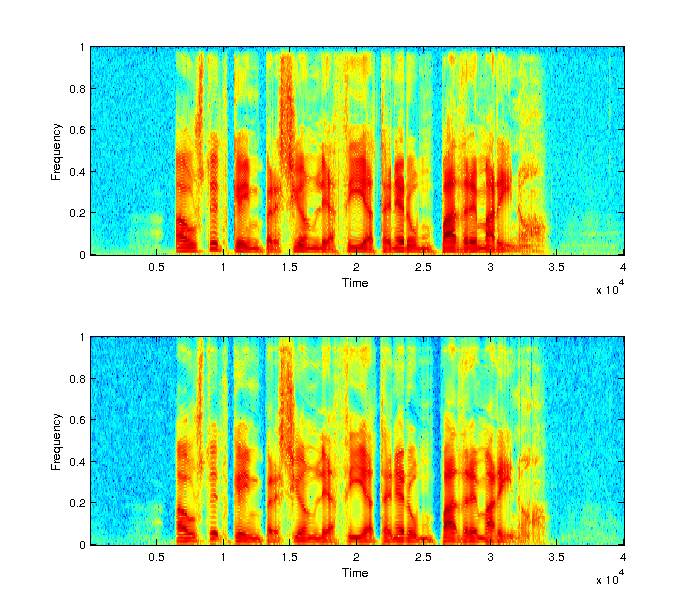
\includegraphics[width=1\textwidth]{img/spectro-ang.png}
	\end{center}
	\caption{\label{angryspec}Spectrogram for the angry emotion of the original file (above) and the synthetic file after resynthesis (below)}
\end{figure}
\begin{figure}[!htb]
	\begin{center}
	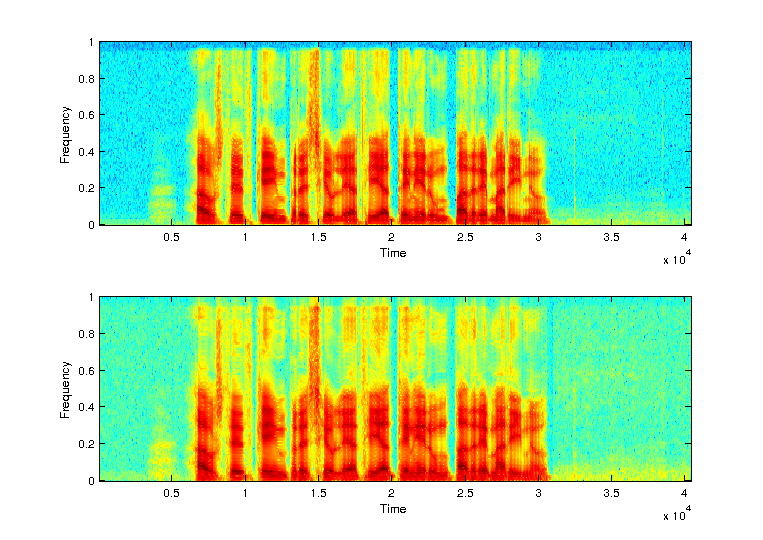
\includegraphics[width=1\textwidth]{img/spectro-sad.png}
	\end{center}
	\caption{\label{sadspec}Spectrogram for the sadness emotion of the original file (above) and the synthetic file after resynthesis (below)}
\end{figure}
Looking into the different configuration files for the different emotions, some little changes can be seen between them. This changes are in the f0 estimation of the analysis, were part the emotion is located (see \ref{emotana}). The rest of the configuration file is the same for all the emotions and it can be also find the parameters that can be extracted in the analysis (can be true or false for all of them) or the ones that will be used in the synthesis. An example of a configuration file can be found in section \ref{anexo}.\\
In this f0 estimation some values can be tuned as:
\begin{itemize}
\item F0\_MIN: Minimum fundamental frequency
\item F0\_MAX: Maximum fundamental frequency
\item VOICING\_THRESHOLD: Voicing threshold with respect to gain in the low-frequency band, so the speech frames under this value will be classified as unvoiced
\item ZCR\_THRESHOLD: Zero-crossings threshold. Speech segments that have more zero crossings than the threshold value are classified as unvoiced
\end{itemize}
So for the male voice the first two values are the almost the same for all the emotions and it is the other two the ones who change in each emotion.
For the female voice this values are totally different than for the male, for example the maximum f0 is bigger than in the case of the male voice.
If all the f0 values obtained after the feature extraction (section \ref{fea}) of all the files used for training are plot, the different f0 for each emotion can be seen in figure \ref{f0estimation} in section \ref{glottexp}.
\subsubsection{HTS Configuration File}\label{htscfile}
In this configuration file the path where the features are going to be extracted is given, and also the streams that are going to be used in the training. The streams are like vectors where all the information of the features of the same type, that will be used in the training, are stored. In the experiment the next streams have been used:
\begin{itemize}
	\item f0: fundamental frequency
	\item lsf1: spectral envelope LSFs
	\item gain1: gain
	\item flow: source LSFs
	\item hnr\_i: harmonic to noise ratio with bands
\end{itemize}
Looking into this file or in the training script it can be seen that the dimension (or size) of this streams is 31 for the lsf (10 for lsf, 10 for the delta coefficients, 10 for the delta-delta coefficients and 1 for the gain), 10 for the flow, 5 for the hnr and 1 for f0.
\subsubsection{Feature Extraction}\label{fea}
The next step is the feature extraction of the audio files that are going to be used in the training. The features that are going to be extracted can be selected in the GlotHMM configuration file.\\
The streams that contains the features will be used in the training for building the voice model, so the features have to represent the voice.
The extracted information for a file is stored in a binary file with cmp extension and is the one that will be used in the training step.
\subsubsection{Training}\label{train}
Once the feature extraction is done the training step can be started. For this a folder with the features (cmp files) and a folder with the time alignment labels is needed.\\
The time alignment labels can be extracted using a front-end. For this a question file will be needed.
The trained is HMM based with five states Gaussian and leaf nodes for the different trees (see section \ref{hmmbased}). For each training two models are generated due to a reclustering is applied to obtain better results. 
Once the training is done and the models are created, one thing that can be done is to realign the training labels using the model that has been created during the training step and train a new model with this realigned labels. This can be done as much times as wanted, and in the case of this project it has be done two times (so we have three rounds) with the male voice in both cases (dependent models y average voice) and with the female voice just with the dependent models due to that with the female average voice a lot of computation time is needed (several weeks).\\
For realigning the labels another HTK tool is used, in this case HSMMAlign see \cite{htkbook} and \ref{htktools}.
So in the end a lot of models are generated due to the reclustering and the realignment. For the dependent models 6 models are created, 2 for reclustering in each training, and 3 trains are performed. In the case of the male average voice the same 6 models are created but the adaptation is done for each emotion with the last one of the reclusterings models so in the end 3 models are generated for each emotion ,so 15 models for the male average voice.\\
As a test is going to be done some sentences for the test need to be synthesized (see section \ref{ttd}) and they have to be the best ones, so before the synthesis this sentences one of the generated models has to be chosen as the best one. This has been done as explained in section \ref{ttd}.
\subsection{Adaptation}\label{adapt}
The adaptation consist in transfer the capabilities of one sepeaker to an average voice (in speaker adaptive training, sat) as is explained in \ref{badapt}.
So basically the steps that has to be followed are the same that with the previous method (section \ref{dpm}), with the difference that this time an average voice model has been build with all the emotions to have a more robust model.\\
In order to do this all the extracted features (cmp files) for the previous method will be placed in the same folder, and the same goes for the time alignment labels, and the SAT (section \ref{at}) has to be set to one in the training script, so there will be only one model (the average).\\
So at this point is where the method differs of the previous one. Now is where the adaptation take place. So an adaptation to this model has been done with every emotion which generates a new model for each emotion.
According with what is told in section \ref{badapt} the type of adaptation is supervised and batch-mode, so different adaptation techniques could have been applied here like MLLR, CMLLR, MAP (see \ref{badapt}) or a combination of some of them like CMLLR + MAP, this is called CSMAPLR (also SMAPLR exist) \cite{analysis-hts-adaptation-junichi}. The adaptation technique that has been used in this Thesis is the CSMAPLR adaptation. For the CMLLR 256 regression tree nodes have been used.
Using MAP after CMLLR improve the average log probability per frame a little bit which leads in a better adaptation. Previously to this MAP technique two iterations of CMLLR have been done to get better results.\\
The CMLLR adaptation can be tuned a little bit with some thresholds which can change the depth of the adaptation, so the emotion level can be tuned with this threshold. Also changing the regression tree nodes can affect the adaptation. As the adaptation has been done using a good amount of data the regression trees can be big and a better node will be selected.\\
For the adaptation all the data of the training for one emotion have been used to replicate the experiment that were done with STRAIGHT, but a big amount of data is not required for a good adaptation.
\subsection{Synthesis}\label{synt}
Once the model are created the process for synthesis is the same in both cases with a little exception when synthesizing labels that have not been seen during the training. In the case of the dependent models (section \ref{dpm}) the models has to be changed to know this new labels, in the case of the adaptation this labels are given when adapting so the new models created new them. For this change a HTK tool is used and it is called HHEd (\ref{htkbook}).\\
So when this is done the first step is to extract the features of the label that is going to be synthesized, as it was explained in \ref{glotthmmvoco} using the models created during the training. This extraction is done with another HTK Tool called HMGenS (\ref{htkbook}). This tool extracts the lsf, flow,logF0 and hnr of the label file.\\
The next step is to extract information of the extracted features to generate the F0, LSF, LSFsource, HNR and GAIN to use the synthesis tool of GlottHMM to generate the audio file.
When synthesizing the global variance (GV) can be used or not. It is supposed to help when the parameters are been generated from the label file with the over-smoothing......AAAAAAAAAAAAalgo por aqui pero no se si lo que escribo esta bien o no. In the case of experiments done sometimes it improved the quality of the generated speech, but in others it introduced some sounds (like whistles). So in some cases the GV was used and in others it was not used. In general with the dependent models it was nos used and with the average voice it was used, but not in all cases.\\ 
Also for the synthesis the HTS engine can be used but requires some transformations to the models.